% ==============================================================================
% capitulos/00-anexoF.tex - Especificación de la API (Swagger & OpenAPI)
% ==============================================================================

\chapter{Especificación de la API: Swagger y OpenAPI}
\label{anexo:especificacion_api}

En este anexo se incluye la documentación técnica detallada de la interfaz de programación (API) del sistema. Se presenta tanto la visualización interactiva generada por Swagger UI como el contrato formal en formato JSON bajo el estándar OpenAPI 3.0.

\section{Documentación Visual (Swagger UI)}
\label{anexo:api_swagger_pdf}
Este documento es la representación gráfica de los endpoints del microservicio. Permite observar los métodos HTTP disponibles, los parámetros de entrada requeridos y los esquemas de respuesta para cada operación del módulo de \textit{Quejoso}.

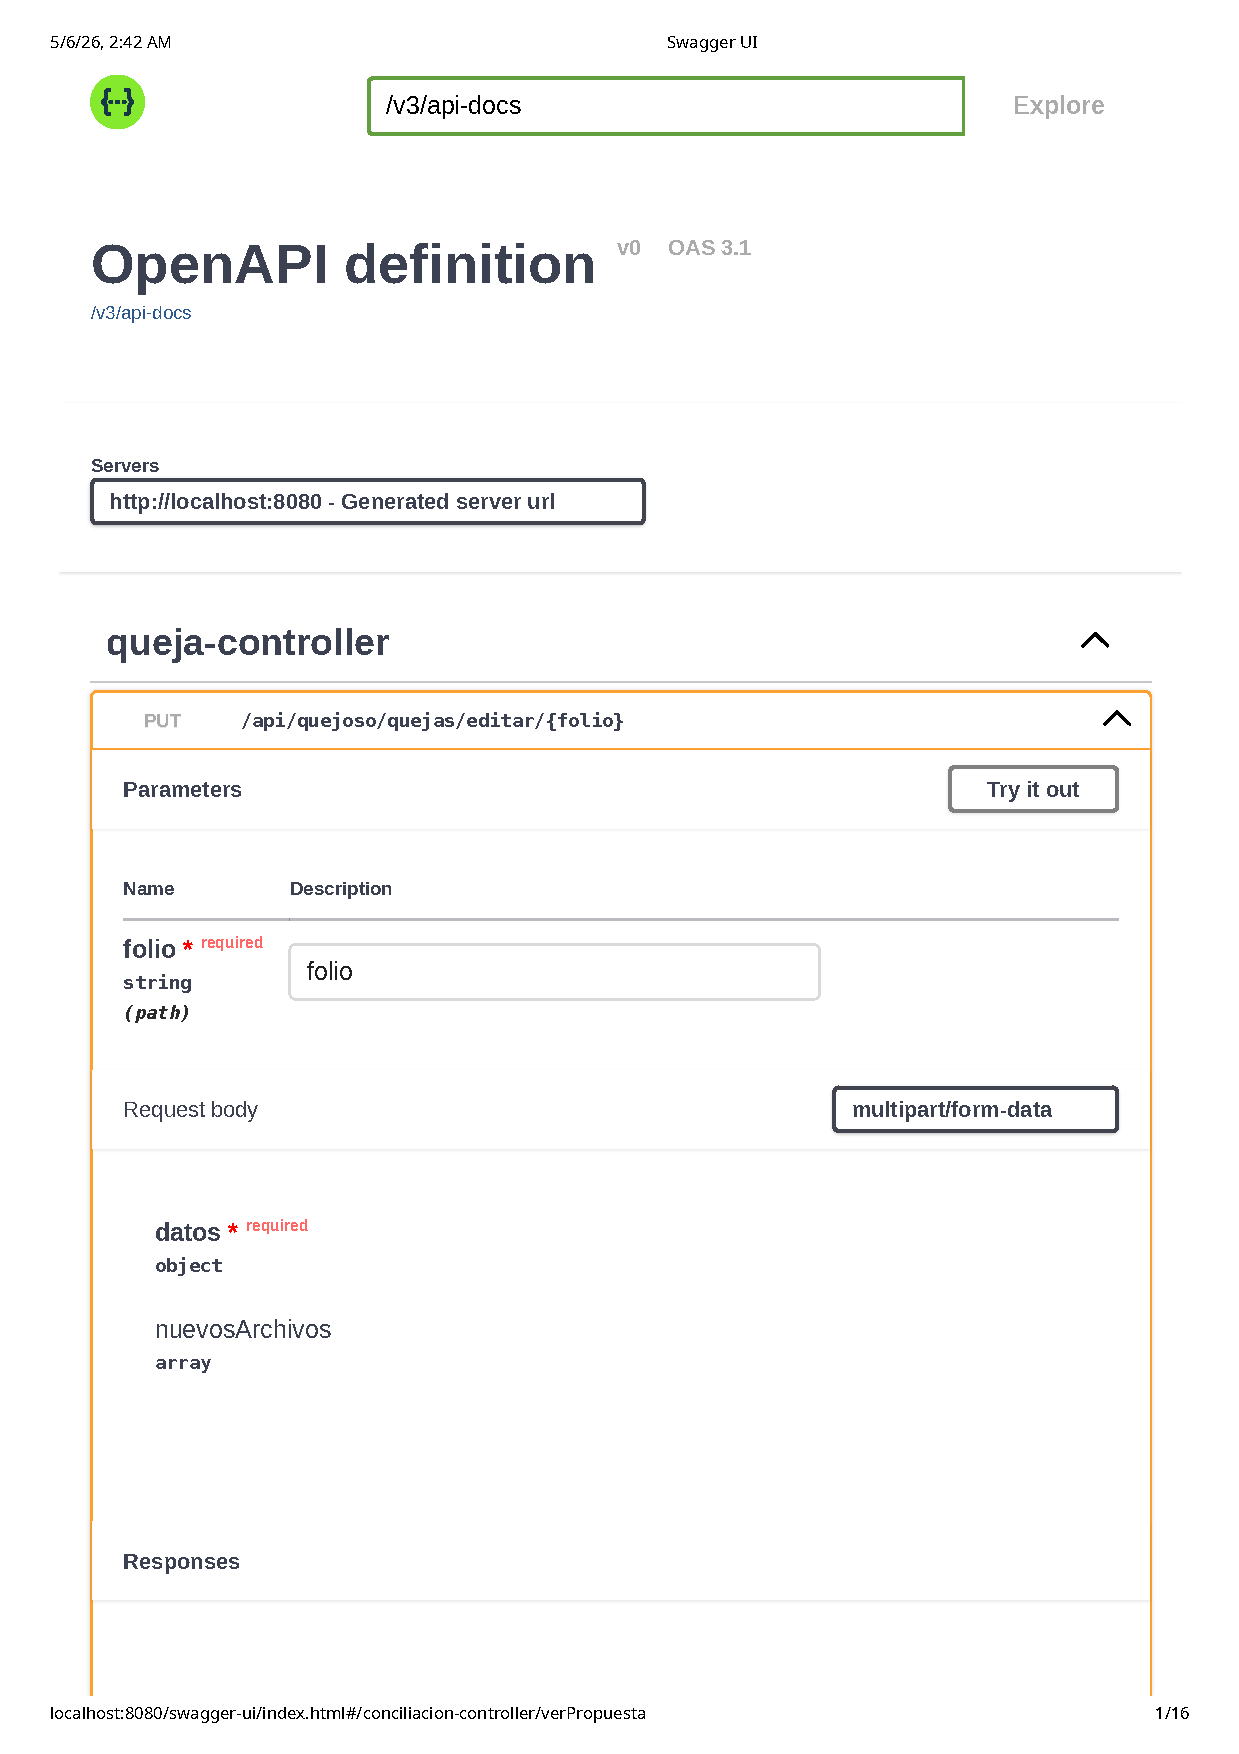
\includepdf[pages=-, frame, scale=0.8, pagecommand={\thispagestyle{plain}}]{APISDOCUMENTACION/quejoso/SwaggerUI-QUEJOSO.pdf}

\section{Contrato Técnico en Formato JSON (OpenAPI)}
\label{anexo:api_json}
A continuación se presenta el archivo de especificación original. Este JSON es el que procesan las herramientas de automatización y el que define la estructura de datos que consume el cliente (Frontend).

\begin{small}
\lstinputlisting[language=json, caption={Archivo de especificación OpenAPI 3.0 del Microservicio Quejoso.}, label={lst:openapi_json}]{APISDOCUMENTACION/quejoso/QUEJOSO.json}
\end{small} % <--- AGREGADO PARA CORREGIR EL ERROR

\section{Resumen de Seguridad de la API}
\label{anexo:api_seguridad}
Como se observa en la especificación, los endpoints críticos están protegidos mediante el esquema de seguridad \textit{Bearer Token} (JWT), asegurando que solo usuarios autenticados puedan acceder a la gestión de expedientes.